\documentclass{article}
\usepackage{amsmath, amssymb}
\usepackage{tikz}
\usetikzlibrary{arrows.meta, decorations.markings}

\begin{document}

\section{Lecture 9: Plan for Class}
Last time:
\begin{enumerate}
    \item Center Manifolds \S 3.2
    \item invariant manifold tangent to center eigenspaces
    \item unlike stable and unstable manifold:
    \begin{enumerate}
        \item cannot define by asymptotic behavior $t\to\pm\infty$
        \item non-unique
        \item not as smooth
    \end{enumerate}
\end{enumerate}

Today:
\begin{enumerate}
    \item Center manifold example
    \item Normal forms \S 3.3
\end{enumerate}

\section{Center manifold example}
This is from the Perko book at page 156.

Let's say that we have the following system
\begin{align*}
    \dot{x}&=x^2y-x^5\\
    \dot{y}&=-y+x^2
\end{align*}
We have an equilibrium point at $(0,0)$. Our Jacobian is 
\[
A = \begin{bmatrix}
    0 & 0\\0 & -1
\end{bmatrix}
\]
Where are eigenvalues are $\lambda=0,-1$ and the eigenvectors are 
\[
v_0 = \begin{bmatrix}
    1\\0
\end{bmatrix},\qquad v_1=\begin{bmatrix}
    0\\1
\end{bmatrix}
\]
On the center subspace $E^c$ at $y=0$, we have 
\[\dot{x}=x^2(0)-x^5=-x^5\]
which tells us that it is stable, and we could use at Lyapunov function $V(x)=\frac{1}{2}x^2$ to show that it is asymptotically stable.

However, $x=0$ is not strictly an invariant set! We could have some weird dynamics around the origin that are not accounted for in this picture.

Let's approximate the center manifold to make arguments as to the stability. We can write 
\begin{align*}
    y&=h(x)=ax^2+bx^3+O(x^4)\\
    \dot{y}&=h'(x)\dot{x}=-h(x)+x^2\\
    \implies&\left(2ax+3bx^3+O(x^3)\right)\left[x^2\left(ax^2+bx^3+O(x^4)\right)-x^5\right]\\
    &=-\left[ax^2+bx^3+O(x^4)\right] + x^2
\end{align*}
From inspection, we see that $a=1$ and $b=0$. So the center manifold is given by 
\[
y=x^2+O(x^4)
\]
Now look at the dynamics on the center manifold (instead of $E^c$). We can write 
\begin{align*}
    \dot{x}&=x^2h(x)-x^5\\
    &=x^2(x^2)-x^5\\
    &=x^4-x^5
\end{align*}
which is actually unstable! Note that this contradicts our earlier reasoning by just looking at $\dot{x}=x^2(0)-x^5=-x^5$.

\begin{figure}[ht]
    \centering
    \vspace{0.5cm}
    \begin{tikzpicture}
        % Main axis line
        \draw[->] (-3,0) -- (3,0);
        
        % Flow arrow on left side (pointing right)
        \draw[->] (-2.5,0) -- (-1.5,0);
        
        % Flow arrow on right side (pointing right)
        \draw[->] (0.5,0) -- (1.5,0);
        
        % Unstable fixed point at origin (open circle)
        \draw[fill=white] (0,0) circle (0.08);
        
        % Label
        \node[below] at (0,-0.15) {$0$};
    \end{tikzpicture}
    \vspace{0.5cm}
    \caption{Phase portrait of $\dot{x}=x^4-x^5$ showing with an unstable fixed point at $x = 0$.}
\end{figure}

\begin{figure}[ht]
    \centering
    \vspace{0.5cm}
    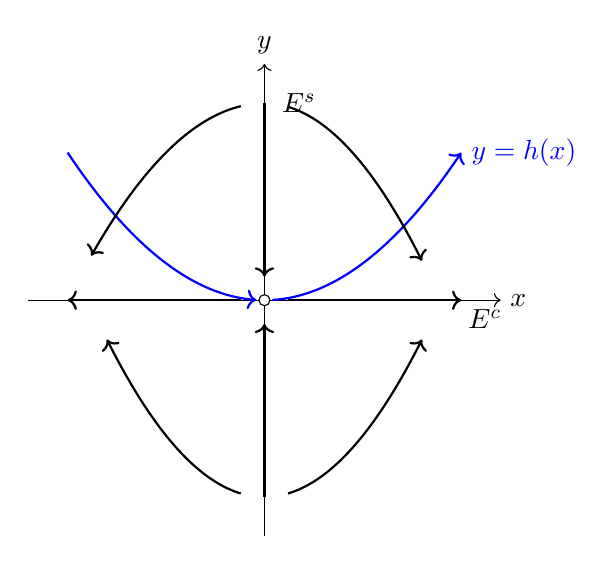
\begin{tikzpicture}
        % Axes
        \draw[->] (-3,0) -- (3,0) node[right] {$x$};
        \draw[->] (0,-3) -- (0,3) node[above] {$y$};

        % Fixed point at origin
        \draw[fill=white] (0,0) circle (0.07);

        % Stable manifold E^s (vertical axis, arrows pointing toward origin)
        \draw[->, thick] (0, 2.5) -- (0, 0.3);
        \draw[->, thick] (0,-2.5) -- (0,-0.3);
        \node[right] at (0.1, 2.5) {$E^s$};

        % Unstable manifold E^c (horizontal axis, arrows pointing away)
        \draw[->, thick] (0.3, 0) -- (2.5, 0);
        \draw[->, thick] (-0.3,0) -- (-2.5, 0);
        \node[below] at (2.8, 0) {$E^c$};

        % Center manifold y = h(x) in blue, upper right and upper left
        \draw[->, blue, thick] plot[domain=0.1:2.5, samples=60] 
            (\x, {0.3*\x*\x}) node[right] {$y = h(x)$};
        \draw[->, blue, thick] plot[domain=-2.5:-0.1, samples=60] 
            (\x, {0.3*\x*\x});

        % Trajectories flowing into origin along stable manifold (white curves)
        % Upper left trajectory
        \draw[->, thick] plot[domain=0.3:2.2, samples=60]
            ({-\x}, {2.5 - 0.4*\x^2});
        % Upper right trajectory  
        \draw[->, thick] plot[domain=0.3:2.0, samples=60]
            ({\x}, {2.5 - 0.5*\x^2});

        % Lower trajectories flowing out
        \draw[->, thick] plot[domain=0.3:2.0, samples=60]
            ({-\x}, {-2.5 + 0.5*\x^2});
        \draw[->, thick] plot[domain=0.3:2.0, samples=60]
            ({\x}, {-2.5 + 0.5*\x^2});

    \end{tikzpicture}
    \vspace{0.5cm}
    \caption{Phase portrait near the equilibrium at $(0,0)$ showing stable manifold $E^s$, unstable manifold $E^c$, and center manifold $y = h(x)$. (Claude generated, so there shouldn't be a crossing of the flow field and the center manifold.)}
\end{figure}

\section{Normal forms \S 3.3}

If we have a linear system, say 
\[
\dot{x}=Ax
\]
we can do a linear change of coordinates with 
\[
x=T\tilde{x}
\]
and then our dynamics become 
\[
\dot{\tilde{x}}=T^{-1}AT\tilde{x}
\]
where $T^{-1}AT$ can be written (if things are nice) as 
\[
T^{-1}AT=\begin{bmatrix}
    \lambda_1 & 0 & \cdots & 0 \\
    0 & \lambda_2 & \cdots & 0 \\
    \vdots & \vdots & \ddots & \vdots \\
    0 & 0 & \cdots & \lambda_n
\end{bmatrix}
\]
But! Things are not always this nice, and we need to use Jordan form, as in
\[
\begin{bmatrix}
    \lambda & 1\\ 0 & \lambda
\end{bmatrix}
\]

\subsection{Motivating example:}
Let's say that we have the following systems
\begin{align*}
    \dot{x}&=x + ax^2 +bxy + cy^2 + O(3)\\
    \dot{y}&=3y + dx^2 + exy+fy^2 + O(3)
\end{align*}
The linear part can be described as 
\[
\begin{bmatrix}
    1 & 0 \\ 0 & 3
\end{bmatrix}
\]
But now our question is: How much can we simplify the quadratic terms with nonlinear change of coordinates? Ideally, we want
\begin{align*}
    x= \tilde{x} + h_1\left(\tilde{x},\tilde{y}\right)\\
    y = \tilde{y} + h_2\left(\tilde{x},\tilde{y}\right)
\end{align*}
where we are ``near identity'' with $h_1,h_2$ being quadratic in $\tilde{x},\tilde{y}$.

\subsection{Resonance terms}

Answer: We can push all quadratic terms to higher order!
\begin{align*}
    \dot{\tilde{x}} = \tilde{x} + O(3)\\
    \dot{\tilde{y}} = 3\tilde{y} + O(3)
\end{align*}
But! Say our system is 
\begin{align*}
    \dot{x}&=x + ax^2 + \cdots\\
    \dot{y}&=2y + dx^2 + \cdot
\end{align*}
Now the best we can do is 
\begin{align*}
    \dot{\tilde{x}} = \tilde{x} + O(3)\\
    \dot{\tilde{y}} = 2\tilde{y} + \tilde{d}\tilde{x}^2 + O(3)
\end{align*}
WHAT!!! It gets worse! Say our system is 
\begin{align*}
    \dot{x}&=x + ax^2 + \cdots\\
    \dot{y}&=\frac{1}{2}y + dx^2 + \cdot
\end{align*}
and now the best we can do is 
\begin{align*}
    \dot{\tilde{x}} &= \tilde{x} + \tilde{c}\tilde{y}^2 + O(3)\\
    \dot{\tilde{y}} &= \frac{1}{2}\tilde{y} + O(3)
\end{align*}
Say it isn't so!

These terms $\tilde{d}\tilde{x}^2,\tilde{c}\tilde{y}^2$ are called ``resonance terms'' and they will be instrumental in allowing us to study certain types of bifurcations.

\subsection{Normal forms}

Let's say that we have the following equation
\[
\dot{x}=Ax + f_2(x) + f_3(x) + \cdots
\]
where $x\in\mathbb{R}^2$, $f_2(x)$ are the quadratic terms, and $f_3(x)$ are the cubic terms.

\subsubsection{Homogeneous functions}

First let's talk about ``homogeneous functions of degree $d$''. These are functions 
\[
f\left(\lambda x_1, \lambda x_2, \ldots, \lambda x_n\right) = \lambda^d f\left( x_1, x_2, \ldots, x_n\right)
\]
where $\lambda$ is only a constant.

Now a homogenous polynomial is like
\begin{itemize}
    \item degree 2: $f(x,y)=x^2 + 4xy+ 2y^2$
    \item degree 3: $f(x,y) = 10x^3-2xy^2 + 3y^3$
\end{itemize}
This is to say, a homogeneous polynomial of degree $d$ is a polynomial where all the terms are of the same degree. The following function 
\[
f(x,y)=x^3 + xy + y
\]
is NOT homogeneous.

\subsubsection{Back to $\dot{x}=Ax+f_2(x)$}

Let
\[
x=y+h_2(x)
\]
where $h_2$ is a homogeneous polynomial of degree 2.

Can we push all terms in $f_2$ to a higher degree? Let's write 
\begin{gather*}
    \dot{y}+Dh_2(y)\dot{y}=\dot{x}\\
    \left(I + Dh_2(y)\right)\dot{y}= A \left(y+h_2(y)\right) + f_2\left(y+h_2(y)\right)
\end{gather*}
We can now write 
\begin{align*}
    \dot{y}&=\left(I + Dh_2(y)\right)^{-1}\left[Ay + Ah_2(y) + f_2(y) + Df_2(y)\cdot h_2(y)\right]\\
    &=\left(I-Dh_2(y)+O(2)\right)\left[Ay + Ah_2(y) + f_2(y) + O(3)\right]\\
    &=Ay + f_2(y) - \left[ Dh_2(y)\, Ay + Ah_2(y) \right] + O(3)
\end{align*}
Cool.

Let's note that we can approximate any matrix $S$ as 
\begin{gather*}
    S=I+ x +\cdots + X^n\\
    XS = x +\cdots + X^n + X^{n+1}\\
    \left(I-x\right)S = I - X^{n+1}\\
    \implies S = \left(I-X\right)^{-1}\left(I-X^{n+1}\right)\\
    S = \left(I-X\right)^{-1}
\end{gather*}
where as $n\to\infty$, it follows that $X^n\to 0$ if eigenvalue are less than 1.

\subsubsection{Getting rid of degree-2 terms}

In order to get ride of all degree-2 terms, we can choose $h_2$ such that 
\[
Dh_2(y)\, Ay-Ah_2(y)=f_2(y)
\]
where it follows (I actually don't know how tho) that 
\[
L_A h_2(y)=Dh_2(y)\, Ay - A h_2(y)
\]
Note that $L_A$ is a linear operator from $H_2\to H_2$ where $H_2$ is the set of all homogeneous degree-2 (vector-valued) polynomials. $H_2$ is essentially a vector space, where we can add and scalar multiply!\footnote{Rowley went on a 5 minute detour catching the audience up to the properties of vector spaces. I will assume the reader knows these properties.}

Hence, the operator $L_A$ such that $L_A h_2=f_2$ exists if and only if $f_2\in\operatorname{Range}(L_A)$. Moreover, we can compute $L_A$ exactly! Cool.

In the book, the authors write
\begin{align*}
    L_A\, h &= \left[A, h\right]\\
    &= ad_A\, h
\end{align*}
where we are denoting a Lie bracket of vector fields.

\subsection{Back to the Resonance example}

We have $\vec{x}=(x,y)$ and 
\[
A=\begin{bmatrix}
    1 & 0 \\ 0 & \lambda
\end{bmatrix}
\]
We can write $L_A$ as 
\begin{align*}
    L_A\, h(x)&=Dh(x)\cdot Ax - A\, h(x)\\
    &=Dh(x)\begin{bmatrix}
        x\\\lambda y
    \end{bmatrix}-\begin{bmatrix}
    1 & 0 \\ 0 & \lambda
\end{bmatrix} h(x)
\end{align*}

Let's note that $H_2$ can be described as 
\[
H_2 = \operatorname{span}\left\{\begin{pmatrix}
x^2\\ 0
\end{pmatrix},\begin{pmatrix}
xy\\ 0
\end{pmatrix},\begin{pmatrix}
y^2\\ 0
\end{pmatrix},\begin{pmatrix}
0\\ x^2
\end{pmatrix},\begin{pmatrix}
0\\ xy
\end{pmatrix},\begin{pmatrix}
0\\ y^2
\end{pmatrix},\right\}
\]
where $\dim H_2=6$. What we want to do now is to write out $L_A\, h(x)=Dh(x)\cdot Ax - A\, h(x)$ for each basis vector in $H_2$ to compute $L_A$.
\begin{align*}
\begin{pmatrix} x^2 \\ 0 \end{pmatrix}&: \quad
\begin{pmatrix} 2x & 0 \\ 0 & 0 \end{pmatrix}
\begin{pmatrix} x \\ \lambda y \end{pmatrix}
-
\begin{pmatrix} 1 & \\ & \lambda \end{pmatrix}
\begin{pmatrix} x^2 \\ 0 \end{pmatrix}
=
\begin{pmatrix} x^2 \\ 0 \end{pmatrix}\\
\begin{pmatrix} xy \\ 0 \end{pmatrix}&: \quad
\begin{pmatrix} y & x \\ 0 & 0 \end{pmatrix}
\begin{pmatrix} x \\ \lambda y \end{pmatrix}
-
\begin{pmatrix} 1 & \\ & \lambda \end{pmatrix}
\begin{pmatrix} xy \\ 0 \end{pmatrix}
= \lambda \begin{pmatrix} xy \\ 0 \end{pmatrix}\\
\begin{pmatrix} y^2 \\ 0 \end{pmatrix}&: \quad
\begin{pmatrix} 0 & 2y \\ 0 & 0 \end{pmatrix}
\begin{pmatrix} x \\ \lambda y \end{pmatrix}
-
\begin{pmatrix} 1 & \\ & \lambda \end{pmatrix}
\begin{pmatrix} y^2 \\ 0 \end{pmatrix}
= (2\lambda - 1) \begin{pmatrix} y^2 \\ 0 \end{pmatrix}\\
\begin{pmatrix} 0 \\ x^2 \end{pmatrix}&: \quad
\begin{pmatrix} 0 & 0 \\ 2x & 0 \end{pmatrix}
\begin{pmatrix} x \\ \lambda y \end{pmatrix}
-
\begin{pmatrix} 1 & \\ & \lambda \end{pmatrix}
\begin{pmatrix} 0 \\ x^2 \end{pmatrix}
= (2 - \lambda) \begin{pmatrix} 0 \\ x^2 \end{pmatrix}\\
\begin{pmatrix} 0 \\ xy \end{pmatrix}&: \quad
\begin{pmatrix} 0 & 0 \\ y & x \end{pmatrix}
\begin{pmatrix} x \\ \lambda y \end{pmatrix}
-
\begin{pmatrix} 1 & \\ & \lambda \end{pmatrix}
\begin{pmatrix} 0 \\ xy \end{pmatrix}
=
\begin{pmatrix} 0 \\ xy \end{pmatrix}\\
\begin{pmatrix} 0 \\ y^2 \end{pmatrix}&: \quad
\begin{pmatrix} 0 & 0 \\ 0 & 2y \end{pmatrix}
\begin{pmatrix} x \\ \lambda y \end{pmatrix}
-
\begin{pmatrix} 1 & 0 \\ 0 & \lambda \end{pmatrix}
\begin{pmatrix} 0 \\ y^2 \end{pmatrix}
= \lambda \begin{pmatrix} 0 \\ y^2 \end{pmatrix}
\end{align*}
This gives us a matrix representation of $LA$ that is 
\[
\begin{pmatrix}
    1 & 0 & 0 & 0 & 0 & 0 \\
    0 & \lambda & 0 & 0 & 0 & 0 \\
    0 & 0 & (2\lambda-1) & 0 & 0 & 0 \\
    0 & 0 & 0 & (2-\lambda) & 0 & 0 \\
    0 & 0 & 0 & 0 & 1 & 0 \\
    0 & 0 & 0 & 0 & 0 & \lambda
\end{pmatrix}
\]
Now if $\lambda\neq0,\frac{1}{2},2$ then $\operatorname{rank}L_A=6$ and we can push all good terms to a higher degree.

However! What if  $\lambda = 0,\frac{1}{2},2$?
\begin{itemize}
    \item If $\lambda=0$, $\operatorname{rank}L_A=4$ and we can't eliminate $\begin{pmatrix}
xy\\ 0
\end{pmatrix},\begin{pmatrix}
0\\ y^2
\end{pmatrix}$
    \item If $\lambda=2$, $\operatorname{rank}L_A=4$ and we can't eliminate $\begin{pmatrix}
0\\ x^2
\end{pmatrix}$
    \item If $\lambda=\frac{1}{2}$, $\operatorname{rank}L_A=4$ and we can't eliminate $\begin{pmatrix}
y^2\\ 0
\end{pmatrix}$
\end{itemize}

\subsection{More general ``resonance'' case}

Let's say we have 
\[
A=\begin{bmatrix}
    \lambda_1 & 0 & \cdots & 0 \\
    0 & \lambda_2 & \cdots & 0 \\
    \vdots & \vdots & \ddots & \vdots \\
    0 & 0 & \cdots & \lambda_n
\end{bmatrix}
\]
where
\[
Ae_i=\lambda_i e_i
\]
and 
\[
h(x)=x_1^{\, m_1}\cdot x_2^{\, m_2} \cdots x_n^{\, m_n}\cdot e_i
\]
Note that $m_1+m_2+\cdots+m_n=M$ where $M$ is the degree.

Then $h(x)$ is an eigenvector of $L_A$ with eigenvalue 
\[
\sum_j m_j\lambda_j-\lambda_j
\]
and whenever this is eigenvalue is equal to $0$, there are resonance terms that can't be eliminated.

\subsection{General procedure}

How could we find the resonance terms that can't be eliminated? First, find $\operatorname{Range}\left(L_A\, h\right)$ for $h\in H_k$, where $H_k$ is the set of homogeneous degree $k$ polynomials. Let $R_k=\operatorname{Range}\left(L_A\right)$ and choose a complement $G_k$ such that 
\[
H_k=R_k\oplus G_k
\]
where the choice of $G_k$ is not unique. It's these terms in $G_k$ that cannot be removed.

\end{document}